\section{Data}
\label{sec:data}
Luminous red galaxies (LRGs) are massive galaxies that populate massive haloes, lack active star formation, and are highly biased tracers of the dark matter gravitational field. A distinct break around 4000 \AA~in the LRG spectrum is often utilized to determine their redshifts accurately. LRGs are widely targeted in previous galaxy redshift surveys \citep[see, e.g.,][]{eisenstein2001spectroscopic, prakash2016sdss}, and their clustering and redshift properties are well studied \citep[see, e.g.,][]{ross2020MNRAS.498.2354R, gilmarin2020MNRAS.498.2492G, bautista2021MNRAS.500..736B, chapman2022MNRAS.516..617C}. 

DESI is designed to collect spectra of millions of LRGs covering the redshift range $0.2<z<1.35$. DESI selects its targets for spectroscopy from the DESI Legacy Imaging Surveys, which consist of three ground-based surveys that provide photometry of the sky in the optical $g$, $r$, and $z$ bands. These surveys include the Mayall $z$-band Legacy Survey using the Mayall telescope at Kitt Peak \citep[MzLS;][]{dey2018overview}, the Beijing–Arizona Sky Survey using the Bok telescope at Kitt Peak \citep[BASS;][]{zou2017project}, and the Dark Energy Camera Legacy Survey on the Blanco 4m telescope \citep[DECaLS;][]{flaugher2015dark}. As shown in Figure \ref{fig:ng}, the BASS and MzLS programmes observed the same footprint in the North Galactic Cap (NGC) while the DECaLS programme observed both caps around the galactic plane; the BASS+MzLS footprint is separated from the DECaLS NGC at DEC $> 32.375$ degrees, although there is an overlap between the two regions for calibration purposes \citep{dey2018overview}. Additionally, the DECaLS programme integrates observations executed from the Blanco instrument under the Dark Energy Survey \citep{abbott2016dark}, which cover about $1130 \deg^{2}$ of the South Galactic Cap (SGC) footprint. The DESI imaging catalogues also integrate the $3.4$ (W1) and $4.6$ $\mu m$ (W2) infrared photometry from the Wide-Field Infrared Explorer \citep[WISE;][]{wise2010AJ....140.1868W, meisner2018RNAAS...2....1M}.  


\subsection{DESI imaging LRGs}
Our sample of LRGs is drawn from the DESI Legacy Imaging Surveys Data Release 9 \citep[DR9;][]{dey2018overview} using the color-magnitude selection criteria designed for the DESI 1\% survey \citep{desi2023sv}, described as the Survey Validation 3 (SV3) selection in more detail in \cite{zhou2022target}. The color-magnitude selection cuts are defined in the $g$, $r$, $z$ bands in the optical and $W1$ band in the infrared, as summarized in Table \ref{tab:ts}. \mr{The selection cuts are developed differently for each imaging survey to reach an almost uniform target surface density, with an average density of $800$ galaxies per square degree covering around $14000$ square degrees, despite different survey efficiency and photometric calibration between DECaLS and BASS+MzLS}. The implementation of these selection cuts in the DESI data processing pipeline is explained in \cite{myers2022}. The redshift distribution of our galaxy sample are inferred respectively from DESI spectroscopy during the Survey Validation phase \citep{desi2023sv}, and is shown via the solid curve in Figure \ref{fig:nz}. \cite{zhou2021clustering} analyzed the DESI LRG targets and found that the redfhit evolution of the linear bias for these targets is consistent with a constant clustering amplitude and varies via $1/D(z)$, where $D(z)$ is the growth factor (as illustrated by the dashed red line in Figure \ref{fig:nz}). 

\begin{figure}
 \centering
 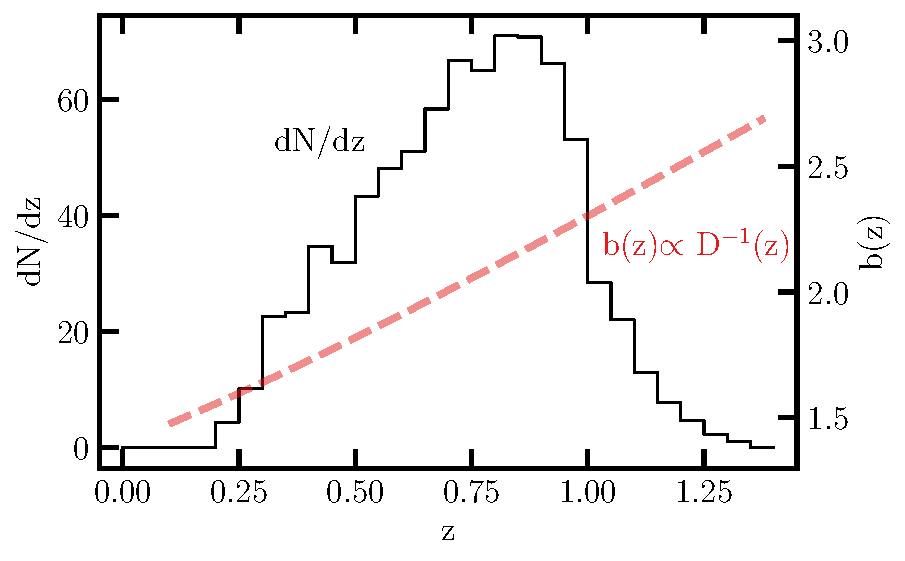
\includegraphics[width=0.45\textwidth]{figures/nz_lrg.pdf}
 \caption{The redshift distribution (solid line) and bias evolution (dashed line) of the DESI LRG targets. The redshift distribution is determined from DESI spectroscopy \citep{desi2023sv}. The redshift evolution of the linear bias is supported by HOD fits to the angular clustering of the DESI LRG targets \citep{zhou2021clustering}, where $D(z)$ represents the growth factor.}
 \label{fig:nz}
\end{figure}

\begin{table*}
\caption{Color-magnitude selection criteria for the DESI LRG targets \citep{zhou2022target}. Magnitudes are corrected for Galactic extinction. The z-band fiber magnitude, $z_{\rm fiber}$, corresponds to the expected flux within a DESI fiber.}\label{tab:ts}
 \centerline{%
 \begin{tabular}{lll}
 \hline
 \hline
 \textbf{Footprint} & \textbf{Criterion} &\textbf{Description}\\
 \hline
 \hline  
 & $z_{\rm fiber} < 21.7$ & Faint limit \\
  DECaLS & $z - W1 > 0.8 \times (r - z) - 0.6$ & Stellar rejection \\
 & $[(g-r >1.3)~{\rm AND}~((g-r) > -1.55*(r-W1) + 3.13)]~{\rm OR}~(r -W 1 > 1.8)$ & Remove low-z galaxies \\
 & $[(r-W1 > (W1 - 17.26)*1.8)~{\rm AND}~(r - W1 > W1 - 16.36)]~{\rm OR}~(r-W1 > 3.29)$ & Luminosity cut \\ 
 \hline
 & $z_{\rm fiber} < 21.71$ & Faint limit \\
 BASS+MzLS & $z - W1 > 0.8 \times (r - z) - 0.6$ & Stellar rejection \\
 & $[(g-r >1.34)~{\rm AND}~((g-r) > -1.55*(r-W1) + 3.23)]~{\rm OR}~(r -W 1 > 1.8)$ & Remove low-z galaxies \\
 & $[(r-W1 > (W1 - 17.24)*1.83)~{\rm AND}~(r - W1 > W1 - 16.33)]~{\rm OR}~(r-W1 > 3.39)$ & Luminosity cut \\ 
 \hline
 \end{tabular}}
\end{table*}

\begin{figure*}
 \centering
 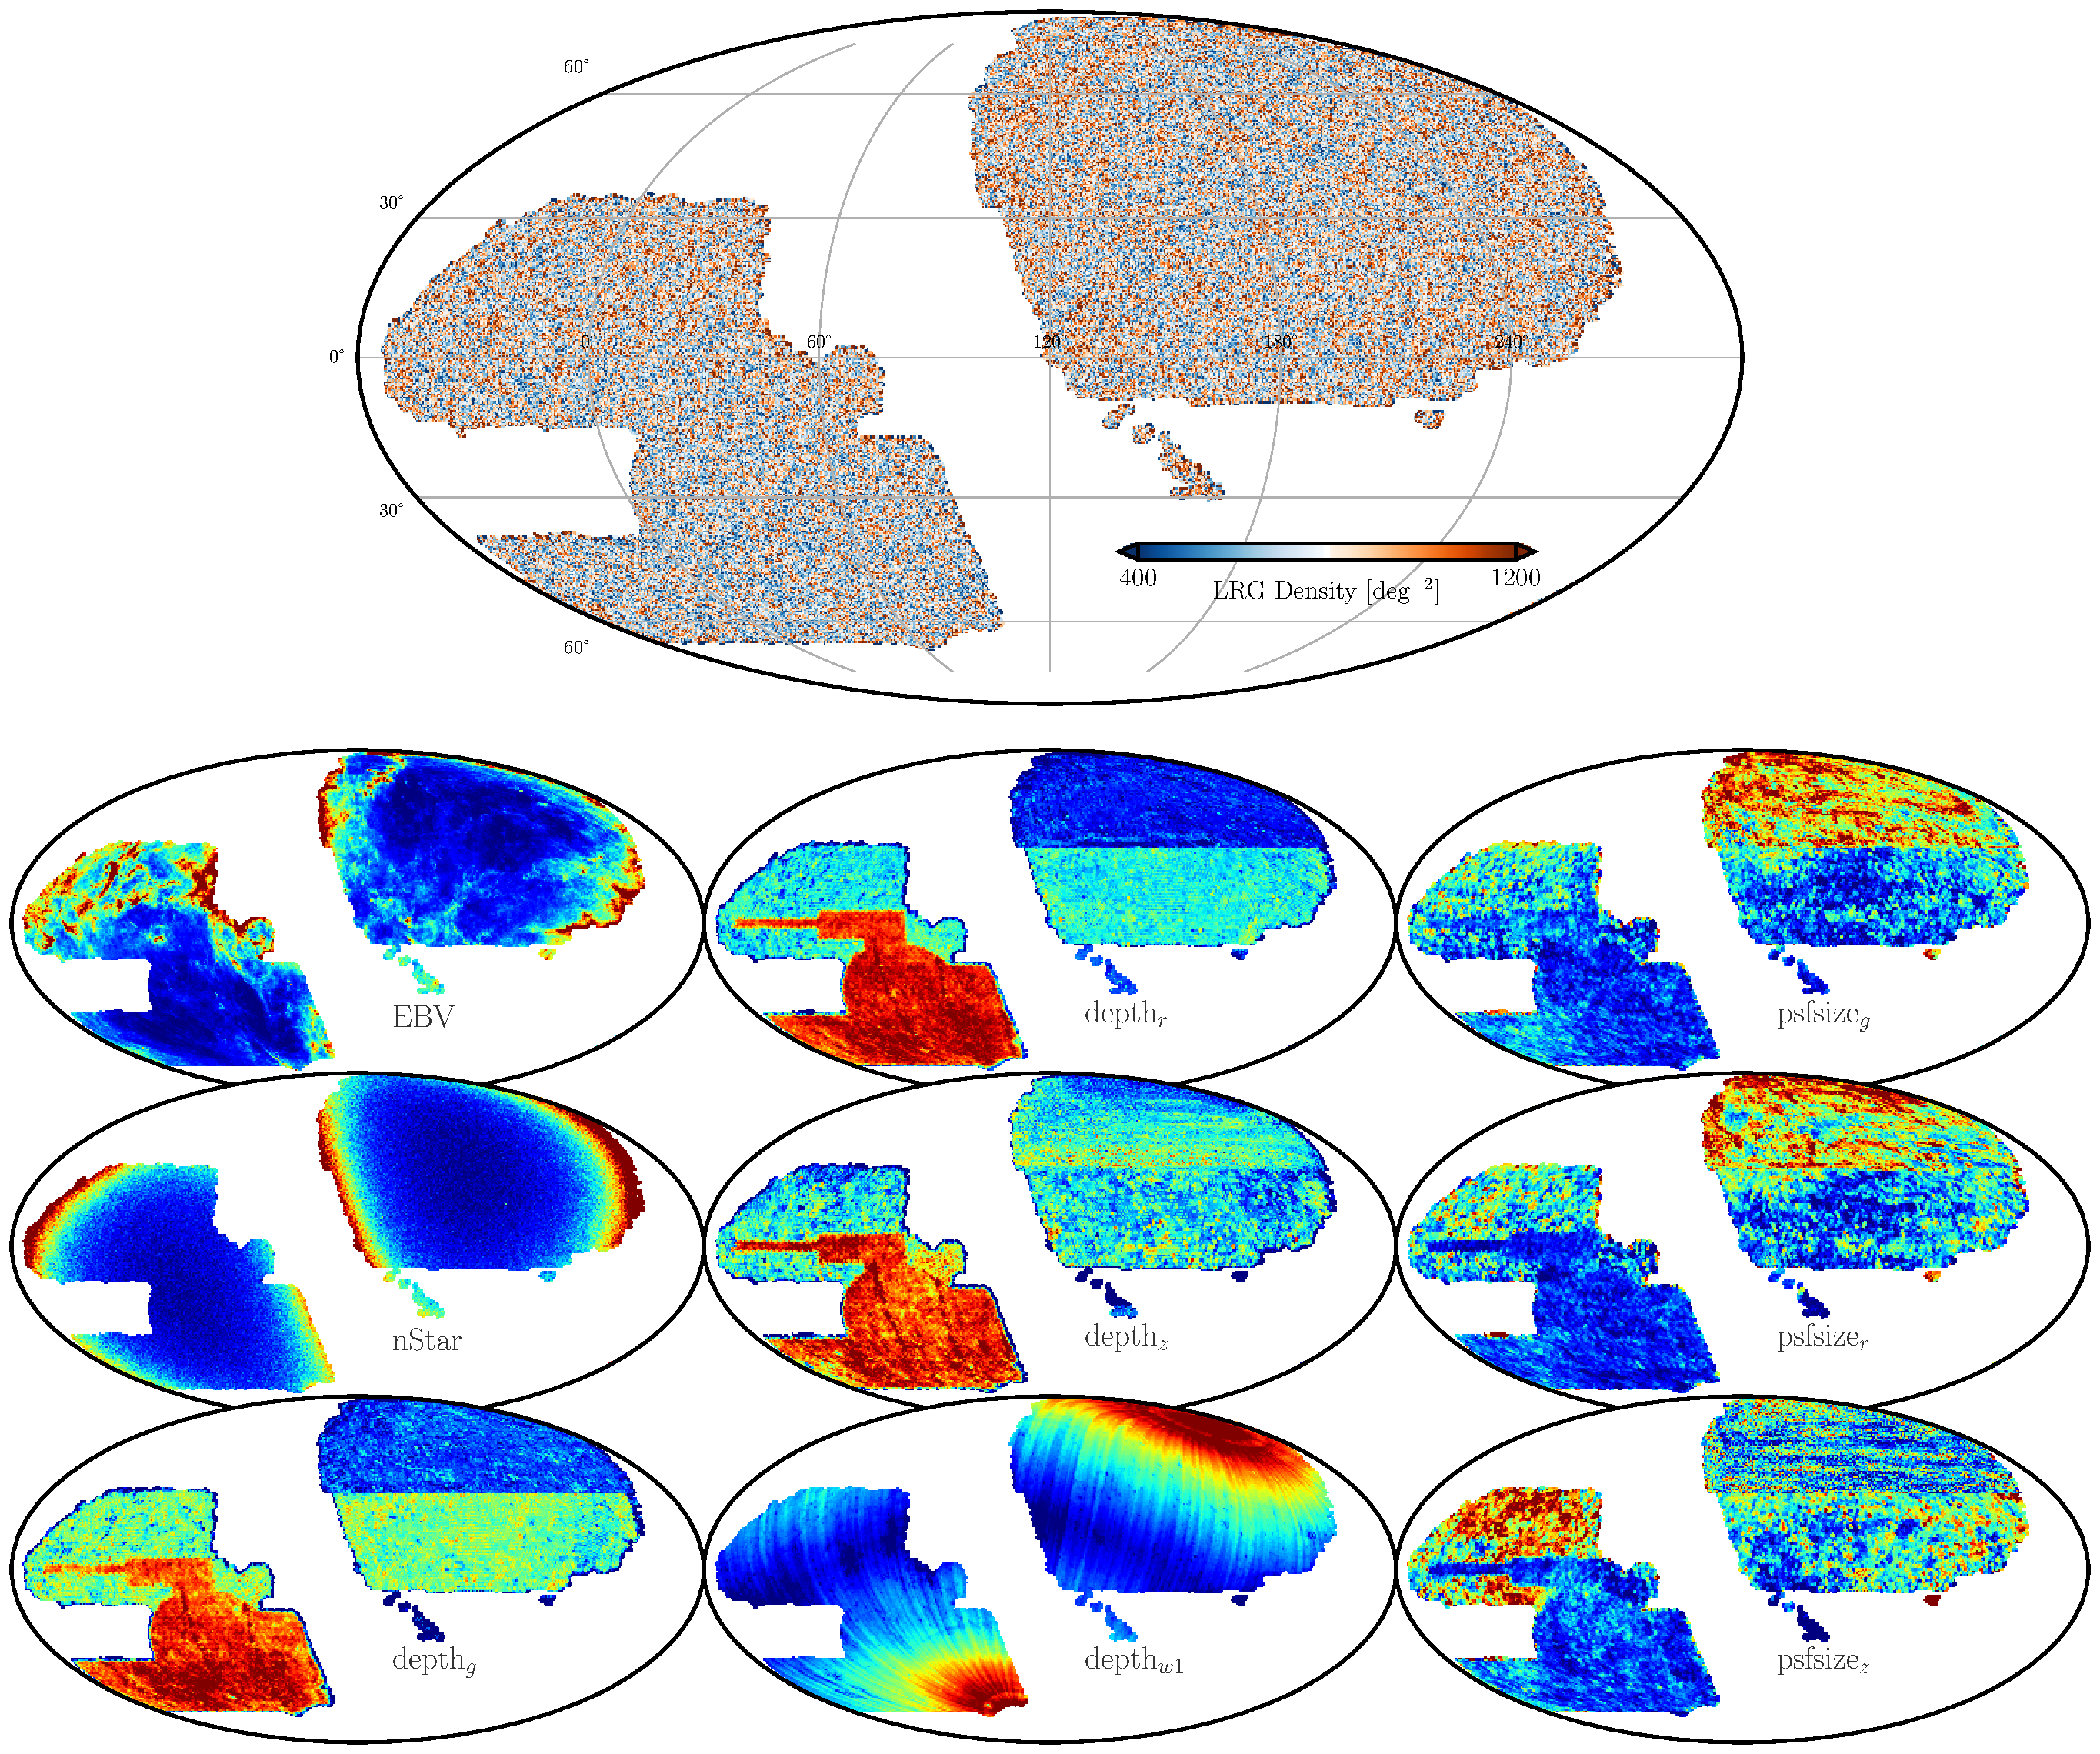
\includegraphics[width=0.99\textwidth]{figures/dr9data.pdf}
 \caption{Top: The DESI LRG target density map before correcting for imaging systematic effects in Mollweide projection. The disconnected islands from the North footprint and parts of the South footprint with declination below $-30$ are removed from the sample for the analysis due to potential calibration issues (see text). Bottom: Mollweide projections of the imaging systematic maps (survey depth, astronomical seeing/psfsize, Galactic extinction, and local stellar density) in celestial coordinates. Not shown here are two external maps for the neutral hydrogen column density and photometric calibration, which are only employed for the robustness tests. The imaging systematic maps are colour-coded to show increasing values from blue to red.}
 \label{fig:ng}
\end{figure*}

The LRG sample is masked rigorously for foreground bright stars, bright galaxies, and clusters of galaxies\footnote{See \url{https://www.legacysurvey.org/dr9/bitmasks/} for maskbit definitions.} to further reduce stellar contamination \citep{zhou2022target}. Then, the sample is binned into \textsc{HEALPix} \citep{gorski2005healpix} pixels at $\textsc{nside}=256$ to construct the 2D density map (as shown in the top panel of Figure \ref{fig:ng}). The LRG density is corrected for the pixel incompleteness and lost areas using a catalogue of random points, hereafter referred to as randoms, uniformly scattered over the footprint with the same cuts and masks applied. \mr{Moreover, the density of galaxies is matched to the randoms separately for each of the three data sections (BASS+MzLS, DECaLS NGC or SGC) so the mean density differences are mitigated. The DESI LRG targets are selected brighter than the imaging survey depth limits, e.g., $g=23.72,~r=23.27,~{\rm and}~z=22.22$ for the median $5\sigma$ detection in AB mag  in the DECaLS region \citep{dey2018overview}; and thus the LRG density map does not exhibit severe spurious fluctuations.}

\subsubsection{Imaging systematic maps}
\cite{zhou2022target} has previously identified nine astrophysical properties as potential sources of imaging systematic errors in the DESI LRG targets. The properties are mapped into \textsc{HEALPix} of \textsc{nside}$=256$. As illustrated by a $3x3$ grid in the bottom panel of Figure \ref{fig:ng}, the maps include local stellar density constructed from point-like sources with a G-band magnitude in the range $12 \leq G < 17$ from the \textit{Gaia} DR2 \citep[see,][]{gaiadr2, myers2022}; Galactic extinction E[B-V] from \cite{schlegel1998maps}; survey depth (galaxy depth in $g$, $r$, and $z$ and PSF depth in W1) and astronomical seeing (psfsize) in $g$, $r$, and $z$. The depth maps have been corrected for extinction using the coefficients adapted from \cite{2011ApJ...737..103S}. In addition to these nine maps, we consider two external maps for the neutral hydrogen column density (HI) from \cite{2016A&A...594A.116H} and photometric calibration in the z-band (CALIBZ) from \mr{CITE} to further test the robustness of our analysis against unknown systematics.

Each imaging map carries its characteristic fluctuations, which correlate with the LRG density map. For instance, large-scale fluctuations can be associated with stellar density, extinction, or survey depth; while small scale-fluctuations can be related to psfsize variations. Some regions of the DR9 footprint are removed from our analysis to avoid potential photometric calibration issues. These regions are either disconnected from the main footprint (e.g., the islands in the NGC with DEC $<-10$) or calibrated using different catalogues of standard stars (e.g., DEC $<-30$ in the SGC). The potential impact of not imposing these declination cuts on the LRG sample and our $\fnl$ constraints is explored in Section \ref{sec:results}. 

\begin{figure}
\centering
 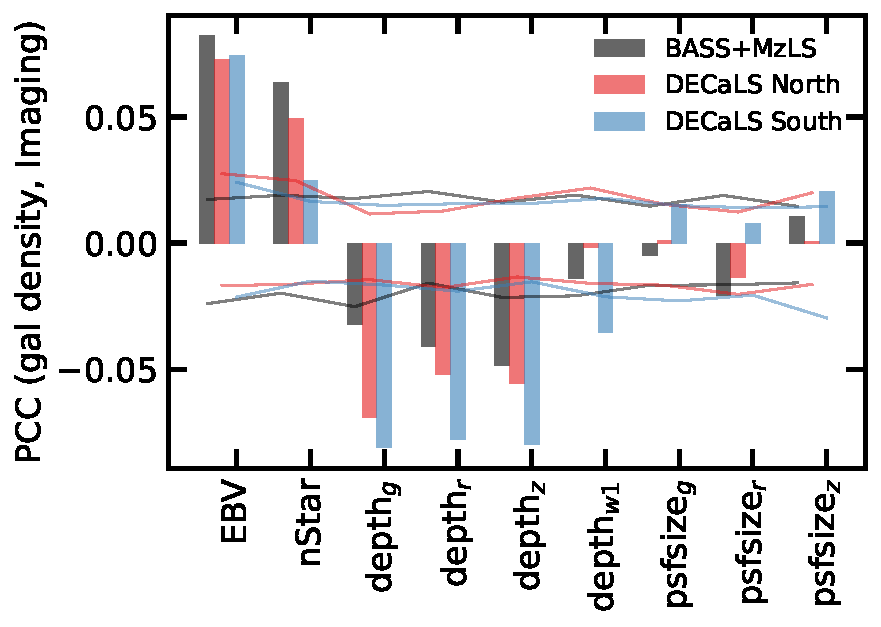
\includegraphics[width=0.45\textwidth]{figures/pcc.pdf} 
 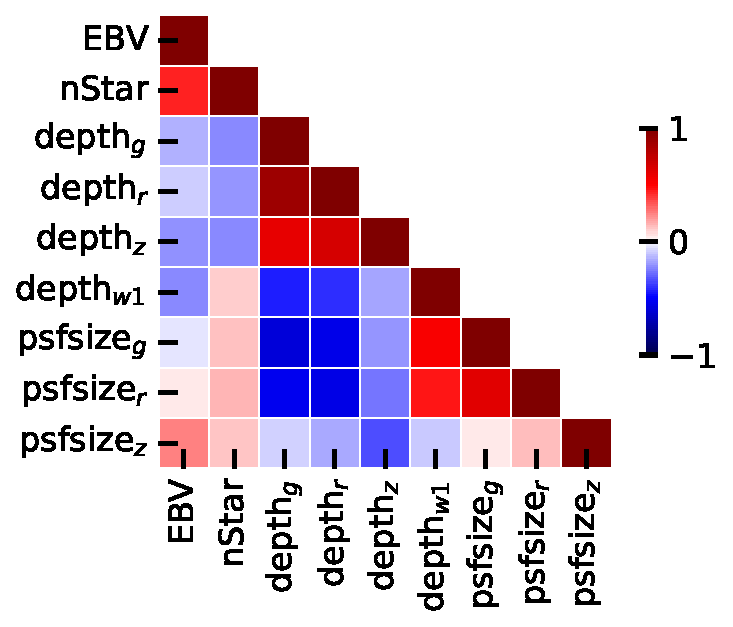
\includegraphics[width=0.45\textwidth]{figures/pccx.pdf}  
 \caption{Top: The Pearson correlation coefficient between the DESI LRG target density and imaging properties in BASS+MzLS, DECaLS North, and DECaLS South. Solid horizontal curves represent the $95\%$ confidence intervals estimated from simulations of lognormal density fields. Bottom: The Pearson correlation matrix of imaging properties for the DESI footprint.}
 \label{fig:pcc}
\end{figure}

Figure \ref{fig:pcc} shows the Pearson correlation coefficient between the DESI LRG target density map and the imaging systematics maps for the three imaging regions (DECaLS North, DECaLS South, and BASS+MzLS) in the top panel. The horizontal curves represent the $95\%$ confidence regions for no correlation and are constructed by cross-correlating 100 synthetic lognormal density fields and the imaging systematic maps. There are statistically significant correlations between the LRG density and depth, extinction, and stellar density. There are less significant correlations between the LRG density and the $W1$-band depth and psfsize in DECaLS South and DECaLS North. Figure \ref{fig:pcc} (bottom panel) shows the correlation matrix among the imaging systematics maps for the entire DESI footprint. Significant inner correlations exist among the imaging systematic maps themselves, especially between local stellar density and Galactic extinction; also, the $r$-band and $g$-band survey properties are more correlated with each other than with the $z$-band counterpart. \mr{We compute the Spearman correlation coefficients as well to assess whether or not the Pearson correlations are impacted by outliers in the imaging data, and find no substantial differences from Pearson.}

The effects of observational systematics in the DESI targets have been studied in great detail \cite[see, e.g.,][]{kitanidis2020imaging, zhou2021clustering, chaussidon2022angular}. There are several approaches for handling imaging systematic errors, broadly classified into data-driven and simulation-based modeling approaches. The general idea behind these approaches is to use the available data or simulations to learn or forward model the relationship between the observed target density and the imaging systematic maps, and to use this relationship, which is often described by a set of \textit{imaging weights}, to mitigate spurious fluctuations in the observed target density. Another techniques for reducing the effect of imaging systematics rely on cross-correlating different tracers of dark matter to ameliorate excess clustering signals, as each tracer might respond differently to a source of systematic error \citep[see, e.g.,][]{giannantonio2014improved}. These methods have their limitations and strengths \citep[see, e.g.,][for a review]{2021MNRAS.503.5061W}.

\subsubsection{Treatment of imaging systematics}
\mr{MR: make this section clear.} In this paper, data-driven approaches, including linear multivariate regression and artificial neural networks, are applied to the data to correct for imaging systematic effects. Both linear and neural network models are trained on each imaging region separately since the Pearson correlation coefficient analysis indicated the level of imaging systematic effects in each region is different, as illustrated in the top panel of Figure \ref{fig:pcc}. 

The linear multivariate model only uses the imaging systematic maps up to the linear power to predict the number counts of the DESI LRG targets in pixel $i$,
\begin{equation}\label{eq:npred}
    \rho_{i} = \log ( 1 + \exp[\textbf{a}.\textbf{x}_{i}]),
\end{equation}
where $\textbf{a}.\textbf{x}_{i}$ represents the inner product between the parameters, $\textbf{a}$, and imaging systematic values for pixel $i$, $\textbf{x}_{i}$. The implementation of Markov Chain Monte Carlo (MCMC) random search from \textsc{emcee} \citep{2013PASP..125..306F} \mr{is used to explore the parameter space by minimizing the negative Poisson log-likelihood between the actual and predicted number counts of targets. No spatial coordinate is included in $\textbf{x}_{i}$ to help avoid over correction, and as a result, the predicted number counts solely reflect the spurious density fluctuations that arise from varying imaging conditions}. The number of pixels is substantially larger than the number of parameters for the linear model, and thus no training-validation-testing split is applied to the data. This aligns with the methodology used for training linear models in previous analyses \citep[see, e.g.,][]{zhou2022target}. \mr{The marginalized mean of the parameters from MCMC are then utilized to compute the imaging weights.}


Our neural network-based mitigation approach uses the implementation of fully connected feedforward neural networks from \cite{rezaie2021primordial}. With the neural network approach, $\textbf{a}.\textbf{x}_{i}$ in Equation \ref{eq:npred} is replaced with $NN(\textbf{x}_{i}|\textbf{a})$, where $NN$ represents the fully connected neural network and $\textbf{a}$ denotes its parameters. The implementation, training, validation, and application of neural networks on galaxy survey data are presented in \cite{rezaie2021primordial}. We briefly summarize the methodology here. 

A fully connected feedforward neural network (also called a \textit{multi-layer perceptron}) is a type of artificial neural network where the neurons are arranged in layers, and each neuron in one layer is connected to every neuron in the next layer. The imaging systematic information flows only in one direction, from input to output. Each neuron applies a non-linear activation function (i.e., transformation) to the weighted sum of its inputs, which are the outputs of the neurons in the previous layer. The output of the last layer is the prediction of the model for the number counts of galaxies. Our architecture consists of three hidden layers with 20 rectifier activation functions on each layer, and a single neuron in the output layer. The rectifier is defined as ${\rm max}(0, x)$ \citep{nair2010rectified}. This simple form of nonlinearity is very effective in enabling deep neural networks to learn more complex, non-linear relationships between the input imaging maps and output galaxy counts.

Unlike linear regression, neural networks are prone to fitting noise, i.e., excellent performance on training data and poor performance on unseen data. Therefore, our analysis uses a training-validation-testing split to ensure that the network is well-optimized and generalizes well to unseen data. Specifically, $60\%$ of the LRG data is used for training, $20\%$ is used for validation, and $20\%$ is used for testing. \mr{The split is performed randomly aside from the locations of the pixels. We test a geometrical split in which neighboring pixels beyond to the same set of training, testing, or validation, but no significant performance difference is observed.} The neural network models are tested on the entirety of the LRG sample with the technique of permuting the choice of the training, validation, or testing sets \citep{arlot2010survey}. The neural networks are trained for up to 70 training epochs with the gradient descent \textsc{Adam} optimizer \citep{2017arXiv171105101L}. The neural network parameters are adjusted iteratively following the gradient of the negative Poisson log-likelihood. The step size of the parameter updates is controlled via the learning rate hyper-parameter, which is initialized with a grid search and is designed to dynamically vary between two boundary values of $0.001$ and $0.1$ to avoid local minima \citep[see, also,][]{2016arXiv160803983L}. At each training epoch, the neural network model is applied to the validation set, and ultimately the model with the best performance on validation is identified and applied to the test set. With the cross-validation technique, the model predictions from the different test sets are aggregated together to form the predicted target density map into \textsc{HEALPix} of \textsc{nside} $=256$. To reduce the error in the predicted number counts, we train an ensemble of 20 neural network models and average over the predictions. The imaging weights are then defined as the inverse of the predicted target density, normalized to unity.

One potential problem that can arise in the data-driven mitigation approach is \textit{over-correction}, which occurs when the corrections applied to the data are too strong that remove the clustering signal and induce additional biases in the inferred parameter. The neural network approach is more prone to this issue compared to the linear approach, due to the increased flexibility. As illustrated in the bottom panel of Figure \ref{fig:pcc}, the significant correlations among the imaging systematic maps may pose additional challenges for modeling these spurious density fluctuations. \mr{Specifically, using highly correlated imaging systematic maps increases the statistical noise in the imaging weights, which elevates the potential for over subtracting the clustering power}. These over-correction effects are identified to have a negligible impact on Baryon Acoustic Oscillations and Redshift Space Distortions \citep{merz2021clustering}; however, they can significantly modulate the galaxy power spectrum on large scales, and thus lead to biased $\fnl$ constraints \citep{rezaie2021primordial, mueller2022primordial}. \mr{Although not explored thoroughly, these issues could limit the detectability of primordial features in the galaxy power spectrum and that of parity violations in higher order clustering statistics \citep{beutler2019primordial, cahn2021test, philcox2022probing}}. Therefore, it is crucial to develop, implement, and apply techniques to minimize and control over-correction, if possible, by reducing the dimensionality of the problem, in the hope of ensuring that the constraints are as accurate and reliable as possible. Our goal is to reduce the correlations between the DESI LRG target density and the imaging systematic maps, while minimizing the chance of over correction.  To achieve this objective, we employ a series of simulations along with statistical methods that involve cross power spectrum and mean galaxy density to identify different sets of the imaging systematic maps: \mr{Santi: Elaborate how these maps are selected}
\begin{enumerate}[itemindent=*]
\item \textbf{Two maps}: Extinction, depth in z.
\item \textbf{Three maps}: Extinction, depth in z, psfsize in r.
\item \textbf{Four maps}: Extinction, depth in z, psfsize in r, stellar density.
\item \textbf{Five maps}: Extinction, depth in z, psfsize in r, neutral hydrogen density, and calibration in z.
\item \textbf{Eight maps}: Extinction, depth in $grzW1$, psfsize in $grz$.
\item \textbf{Nine maps}: Extinction, depth in $grzW1$, psfsize in $grz$, stellar density.
\end{enumerate}

\mr{Edmond: You can comment a bit on the different combinations; why / how do you decide which combination we want ? (maybe just say that it is explained below, your sentence on visual inspection)}
\mr{Alex: Throughout—I think it would be clearer if you always referred to every method with 2 labels, “[linear/nonlinear] [map name]”.} We emphasise that these sets are established prior to examining the auto power spectrum of the LRG sample. The auto power spectrum measurements are \textit{unblinded} only after our mitigation methods passed our rigorous tests for residual systematics. To start, we will use the linear model and two maps (extinction and depth in z), which is the most conservative method in terms of both the model flexibility and the number of parameters. We clean the sample using the imaging weights obtained from \textit{linear two maps}. We find that the linear two maps approach mitigates most of the spurious fluctuations in the LRG density and reduces the cross-correlations between the LRG density and the imaging systematic maps, except for the trends against psfsize in the r and z bands. Adding the r-band psfsize improves the linear model performance such that the cross correlations are similar to those obtained from linear eight maps, which indicates no further information can be extracted from eight maps. Therefore, we identify extinction, depth in z, and psfsize in r (\textit{three maps}) as the primary sources of systematic effects. Then, we adapt \textit{neural network three maps} to model non-linear systematic effects, and find that the neural network-based weights significantly reduce the cross correlations and spurious density fluctuations. As explained in Section \ref{sec:method}, we consider neural network with four, five, and nine maps to further test for the robustness of our cleaning methods.


\subsection{Synthetic lognormal density fields}\label{ssec:mocks}
Density fluctuations of galaxies on large scales can be approximated with lognormal distributions \citep{coles1991}. Unlike N-body simulations, simulating lognormal density fields is not computationally intensive, and allows quick and robust validation of data analysis pipelines. These mocks are therefore considered useful for our study since the signature of local PNG appears on large-scales and small scale clustering is not used. The package \textsc{FLASK} \citep[Full-sky Lognormal Astro-fields Simulation Kit;][]{Xavier_2016} is employed to generate ensembles of synthetic lognormal density maps that mimic the bias, redshift, and angular distributions of the DESI LRG targets, as illustrated in Figure \ref{fig:nz} and \ref{fig:ng}. Two universes with $\fnl=0$ and $76.92$ are considered. A set of 1000 realizations are produced for every $\fnl$. \mr{The analysis adapts a fiducial cosmology from a flat $\Lambda$CDM universe, including one massive neutrino with $m_{\nu}=0.06$ eV, Hubble constant $h = 0.67$, matter density $\Omega_{M}=0.31$, baryon density $\Omega_{b}=0.05$, and spectral index $n_{s}=0.967$. The amplitude of the matter density fluctuations on a scale of $8 h^{-1} \text{Mpc}$ is set as $\sigma_{8}=0.8225$.} The same fiducial cosmology is used throughout this paper unless specified otherwise. \mr{Santi: how sensitive is the fnl signal to the choice of fiducial cosmology.}

\subsubsection{Contaminated mocks}
The linear model is employed to introduce synthetic spurious fluctuations in the lognormal density fields. The motivation for choosing a linear contamination model is to assess how much of the clustering signal can be removed by applying more flexible and rigorous models, based on neural networks, for correcting imaging systematic effects. The parameter space of the linear model is explored using MCMC, from the relationship between the LRG sample and the imaging systematic maps. The MCMC process is executed separately on each imaging survey using only \textit{three maps} (extinction, depth in z, and psfsize in r) as $\textbf{x}_{i}$. The imaging selection function for contaminating each simulation is uniquely and randomly drawn from the parameter space probed by MCMC, and then the results from each imaging survey are combined to form the DESI footprint. The same contamination model is used for both the $\fnl=0$ and $76.92$ simulations.

Similar to the imaging systematic treatment analysis for the DESI LRG targets, the neural network methods with various combinations of the imaging systematic maps are applied to each simulation, with and without PNG, and with and without systematics, to derive the imaging weights. Section \ref{sec:method} presents how the simulation results are incorporated to calibrate $\fnl$ biases due to over-correction. 